\documentclass[11pt]{article}
\usepackage[english]{report}
\usepackage{titling}
\setlength{\droptitle}{-3em}

\title{Floating Vehicle for Environmental \\ Cleaning of Large Liquid Masses}
\author{Anton Eriksson (aner0164@student.umu.se) \\
  Emelie Nordlinder (emelienordlinder@gmail.com) \\
  Jenny Bergman (jebe0070@student.umu.se) \\
  Jesper Vesterberg (jesper.vesterberg@umu.se) \\
  Joel Vedin (jove0027@student.umu.se) \\
  Johan Olovsson (joed0049@student.umu.se) \\
Rasmus Nyman (rany0004@student.umu.se)}

\date{\today}

\begin{document}
\begin{titlepage}
  \maketitle
  \thispagestyle{fancy}
  \lhead{
    Department of Physics\\
    Umeå University
  }
  \rhead{\today}

\begin{figure}[H]
   \centering
   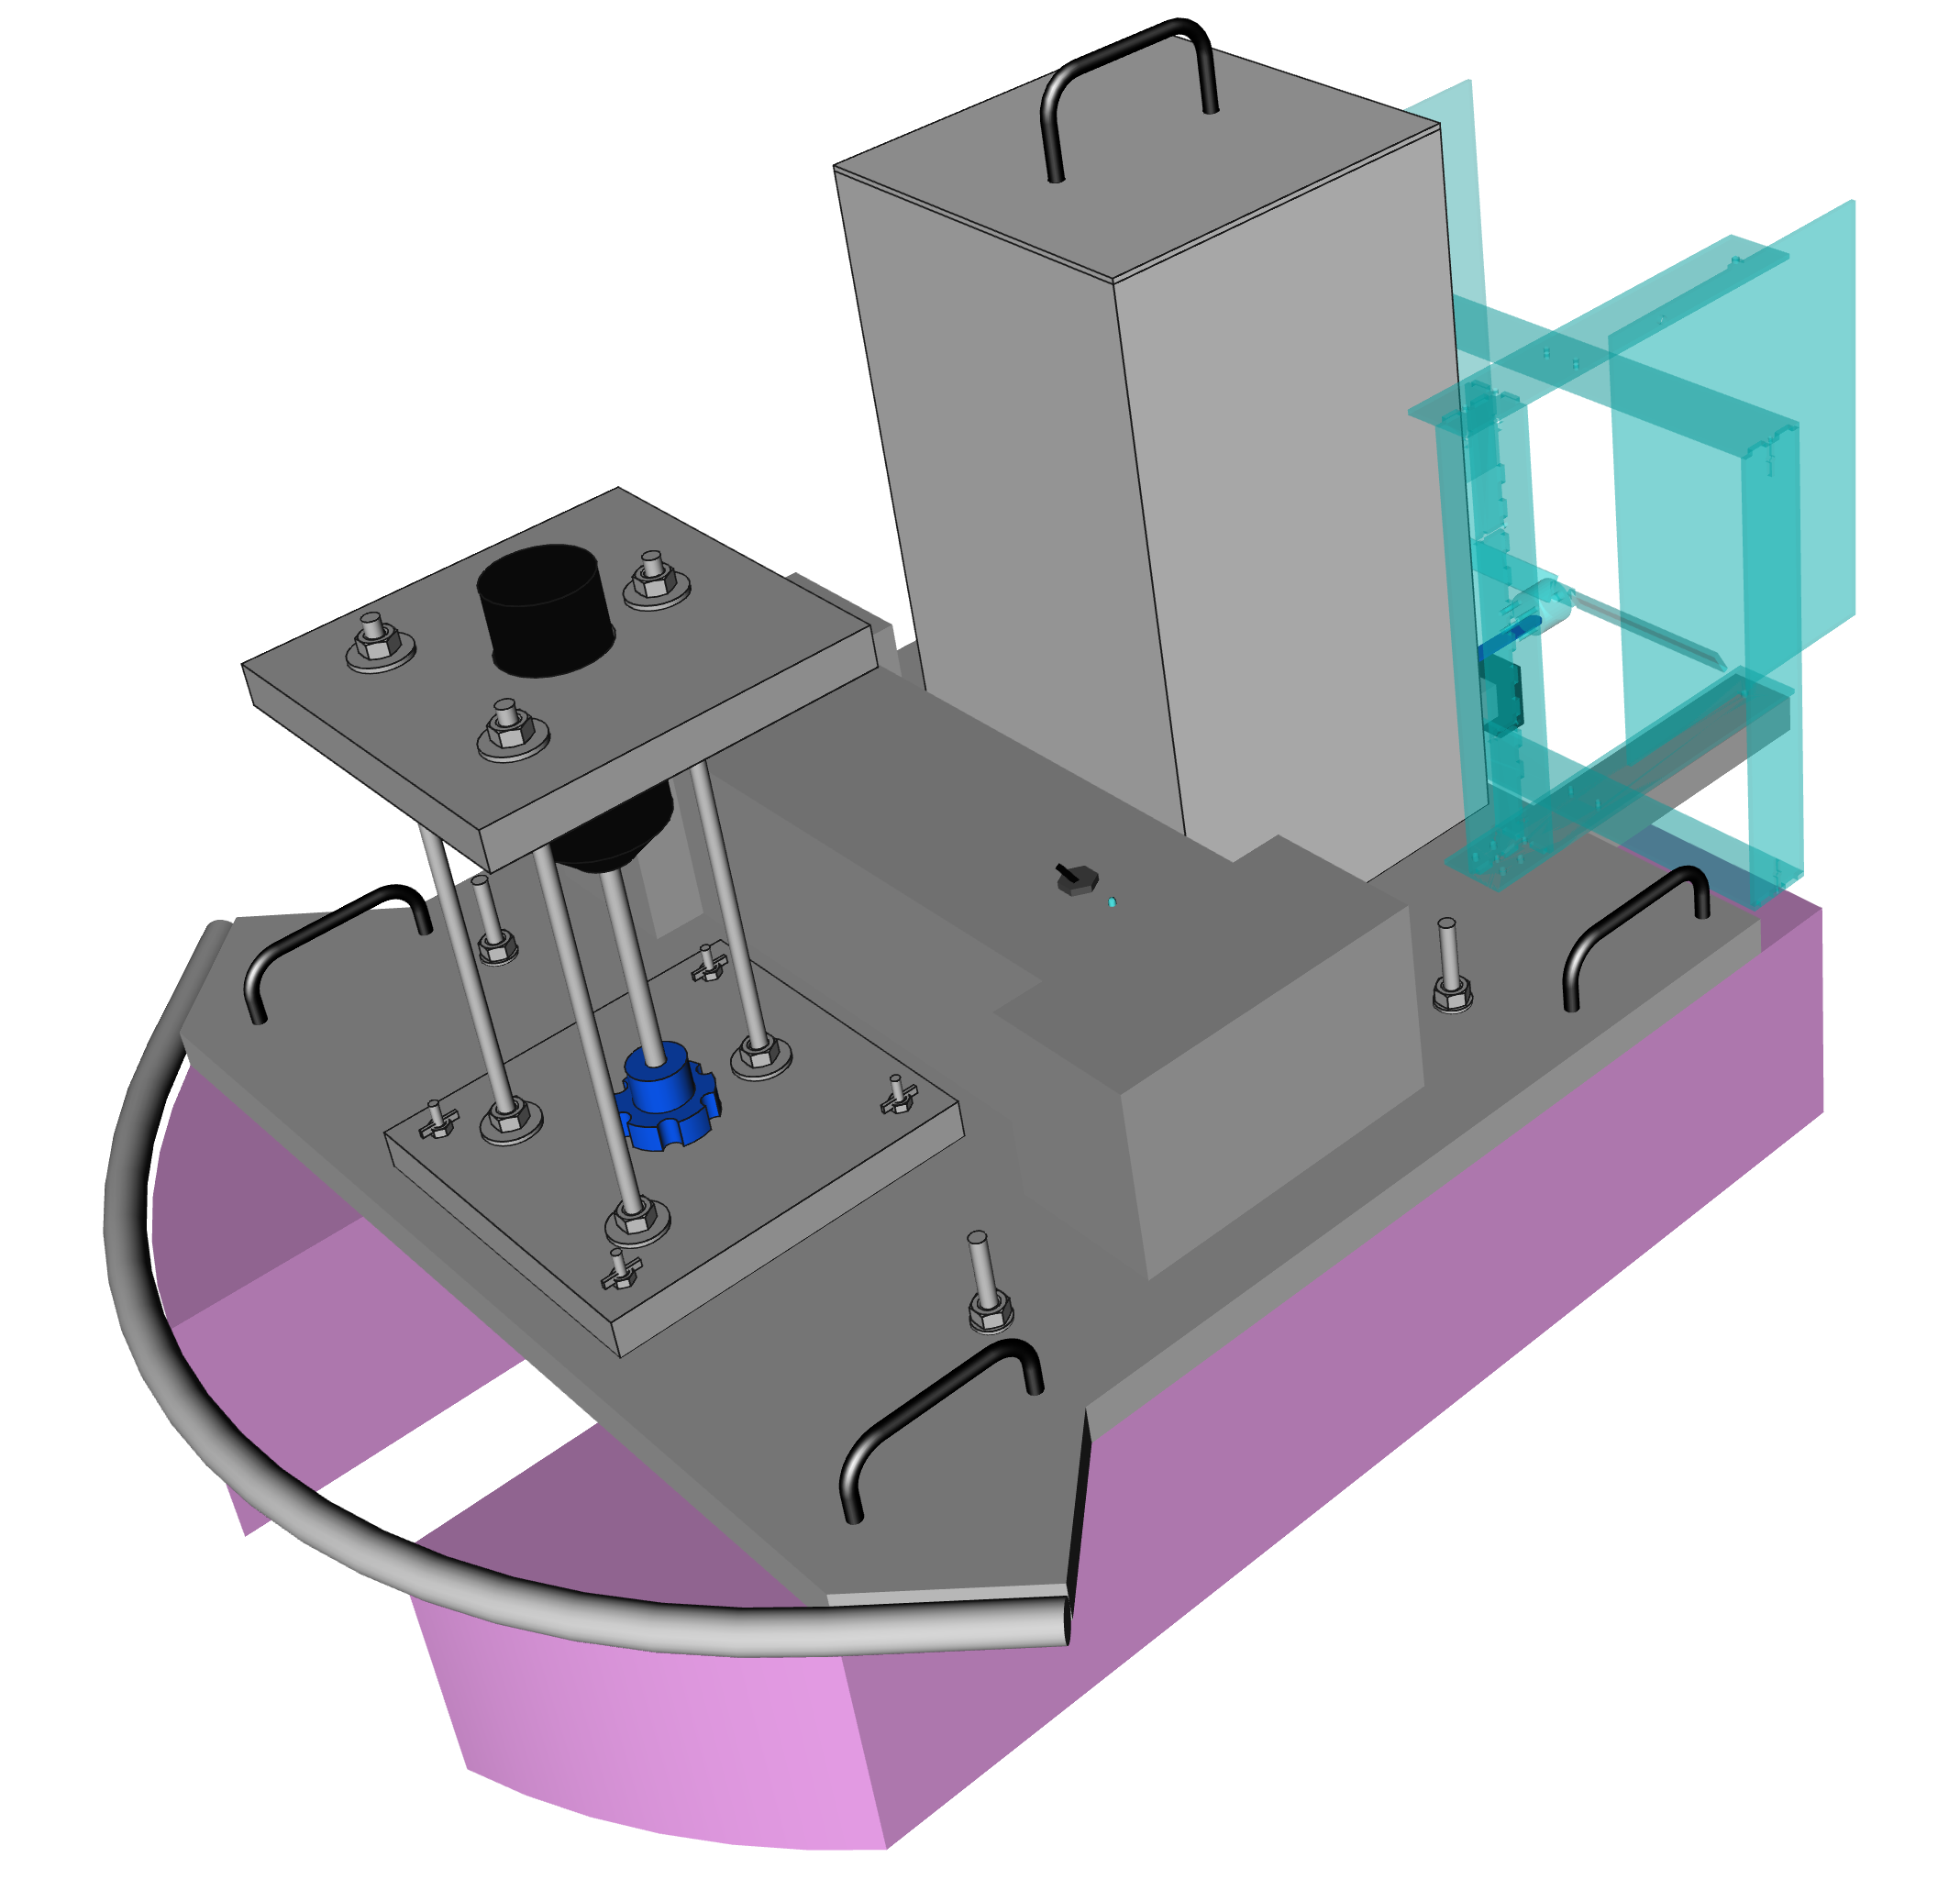
\includegraphics[width=.5\textwidth]{front_box_off_2}
   \label{fig:controller_front}
\end{figure}

  \begin{abstract}
    \noindent
    SpinChem has developed a rotating bed reactor (RBR) which can be used to
    clean fluids of particles or chemicals. This report describes a floating
    vehicle for mobilizing the RBR, which allows for cleaning large bodies of
    water via remote control. The vehicle uses battery-powered propulsion and
    rotation of the RBRs and can be operated at large distances from the
    operator. Emphasis has been placed on ease of transportation and cost
    effectiveness of the construction. Tests show that a simulated water
    contaminant can be effectively cleaned with our vechile. Future development
    could include autonomous deployment, and adapting the vehicle for more
    specialized purposes, such as algae harvesting. There is also a possibility
    to produce an lighter weight version of the vehicle, using more advanced
    production methods.
  \end{abstract}

  \cfoot{
    Design-Build-Test\\
    Supervisor: Krister Wiklund
  }
\end{titlepage}

\lhead{\thetitle}
\rhead{\today}
\cfoot{\thepage}

\section*{\centerline{Project group}}

%\todo{Ska tabelltexten vara med?}

\centerline{Umeå University}
\FloatBarrier
\begin{table}[H]
\center
%\caption{The project group together with responsibilities and e-mail adresses.}
\begin{tabular}{l p{0.28\linewidth} l}
\toprule
\rowcolor{lightgray}
Name & Responsibility & E-mail\\
\midrule
Anton Eriksson & Scrum master & ener0164@student.umu.se\\
\midrule
Emelie Nordlinder & Team member & emno0046@student.umu.se\\
\midrule
Jenny Bergman & Team member & jebe0070@atudent.umu.se\\
\midrule
Jesper Vesterberg & Project leader & jesper.vesterberg@umu.se\\
\midrule
Joel Vedin & Team member & jove0027@student.umu.se\\
\midrule
Johan Olovsson & Team membert & joed0049@student.umu.se\\
\midrule
Rasmus Nyman & Team member & rany0004@student.umu.se\\
\bottomrule
\end{tabular}
%\label{tab:var}
\end{table}

\centerline{\textbf{Customer:} SpinChem\textsuperscript{\textregistered} AB}

\centerline{\textbf{Customer contact person:} Erik Löfgren, erik@spinchem.com}

\centerline{\textbf{Supervisor:} Krister Wiklund}


\clearpage

\tableofcontents
\clearpage

\section{Introduction}

SpinChem has developed a rotating bed reactor (RBR) for chemical and medicinal applications. This device is usually mounted in a stationary set-up in a controlled environment. This report describes a method, and platform, for mobilizing the RBR for usage in various bodies of fluid. More specifically, there was an interest in investigating if the vehicle, together with the RBR, could be used for cleaning polluted waters in our environment, e.g. heavy metal polluted lakes or ponds created by the mining industry. The project hinged on the ability to construct a floating platform which could deliver power, mobility, and remote control for one or more RBRs. As the application was for use in water, all electronics needed to be suitably waterproof, and overall, a desire was for the design to be easily replicable, such that as many products as possible are ''of the shelf'' products. 

Another part of this project was to use a RBR and evaluate the capacity of different materials to adsorb metal ions, such as Cu2+-ions and Zn2+-ions, in polluted water over time. All work was done during the course Design-Build-Test, and the constraints were one semester, with seven engineering students working part time, and a budget of around 10.000 SEK provided from Umeå University.
\clearpage
\section{Floating Platform}
The floating platform, depicted in
\cref{fig:floatingPlatform}, is the main structure of the built vehicle.
It is a baffle of glulam wood, with two pieces of XPS cell foam as
pontoons, where all the components are attached. It can keep a mass of
around 20~kg above water with margins.

In the middle of the platform two symmetrical holes with fittings was
been made, in which the RBR modules can be attached or detached. In the front of the platform a large rounded bumper helps with deflection of head on collisions. It also creates a distance between the platform and
any side obstacles, which helps maneuvering in tight spots and sharp corners. In the
middle of the platform the majority of the electronics has been placed. The electronics and the RBR modules have acrylic
protection covers, protecting the equipment from small splashes of water and rain.

\begin{figure}[h]
   \centering
   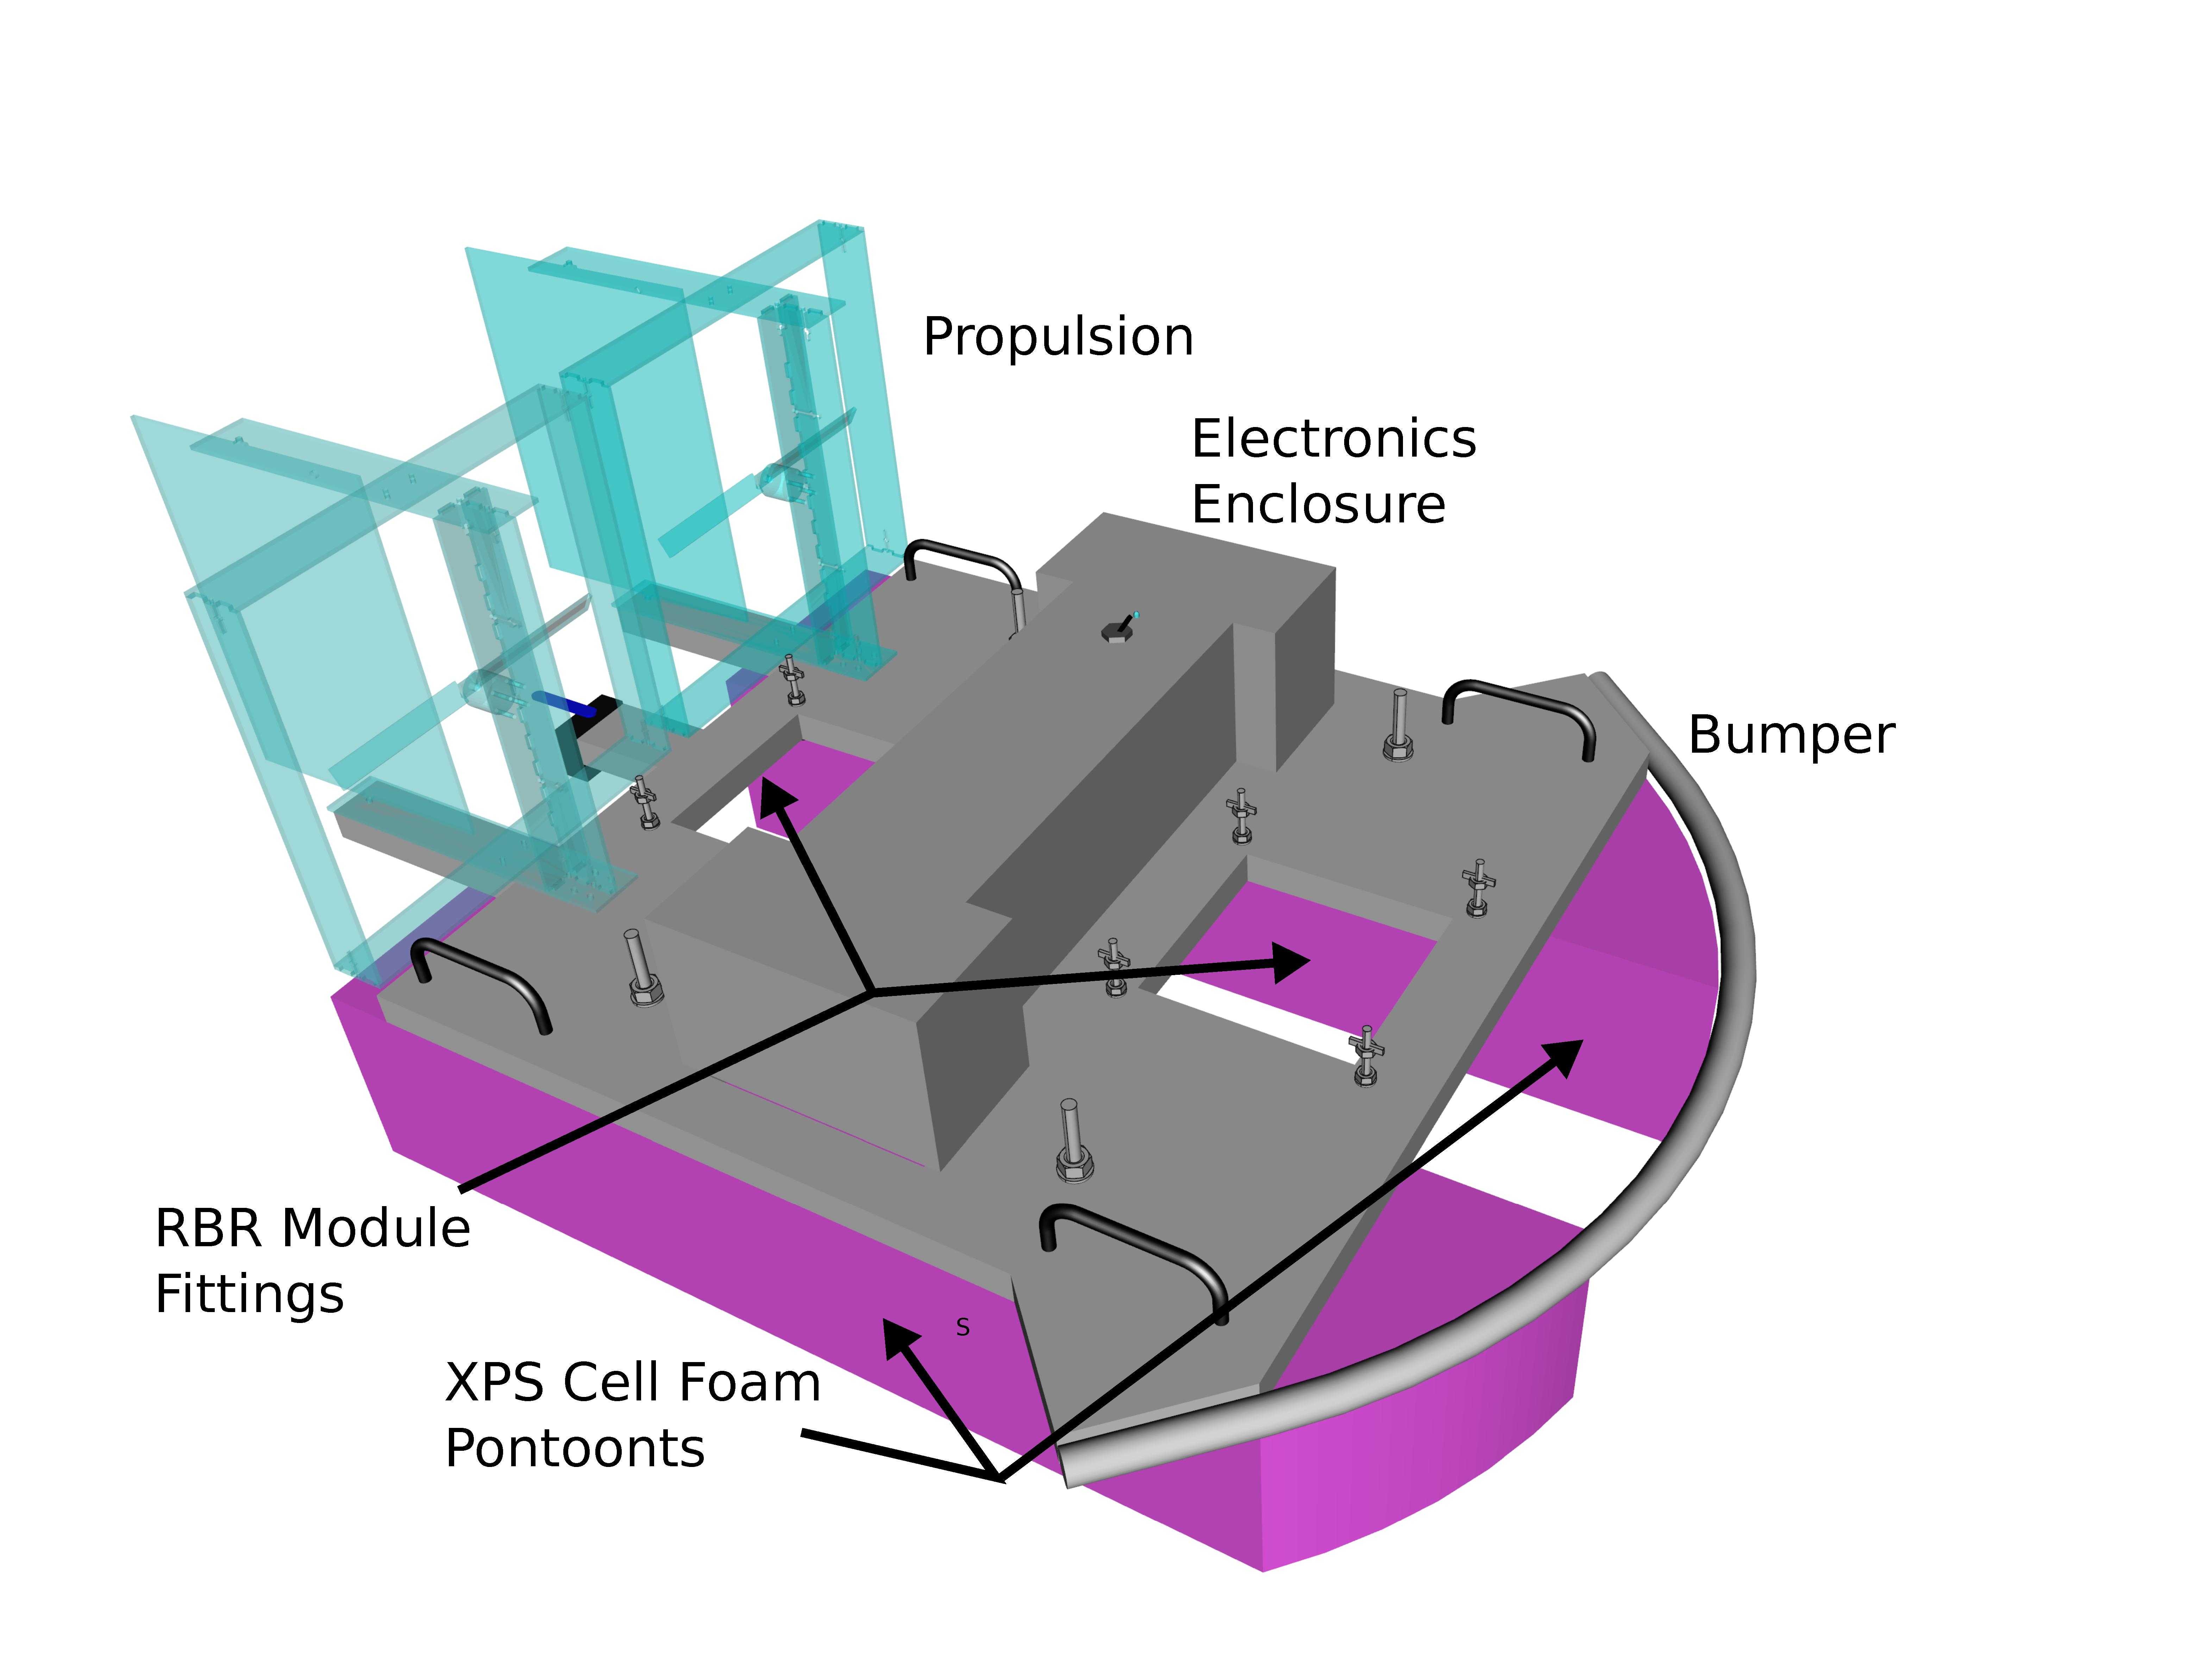
\includegraphics[width=.75\textwidth]{platformWithNotes.eps}
   \caption{The floating platform without the RBR modules installed.}
   \label{fig:floatingPlatform}
\end{figure}

\subsection{RBR module}
The RBR module, seen in fig. \ref{fig:rbr-module} consist of two baffles, separated by three adjustable threaded
rods. The upper mounted baffle is constructed with a modified hand-held screwdriver. The lower mounted
baffle has a PTFE shaft guide mounted for a RBR axle. A shaft can then be driven through the shaft guide and be attached to the screwdriver, in order to drive the RBRs under water. The lower mounted baffle has an
additional baffle which goes down into the water just above where a mounted RBR
will be situated. This baffle prevents the formation of large vortices above the RBR. 

\begin{figure}[H]
  \centering
  \textbf{RBR module}
  \par\medskip
  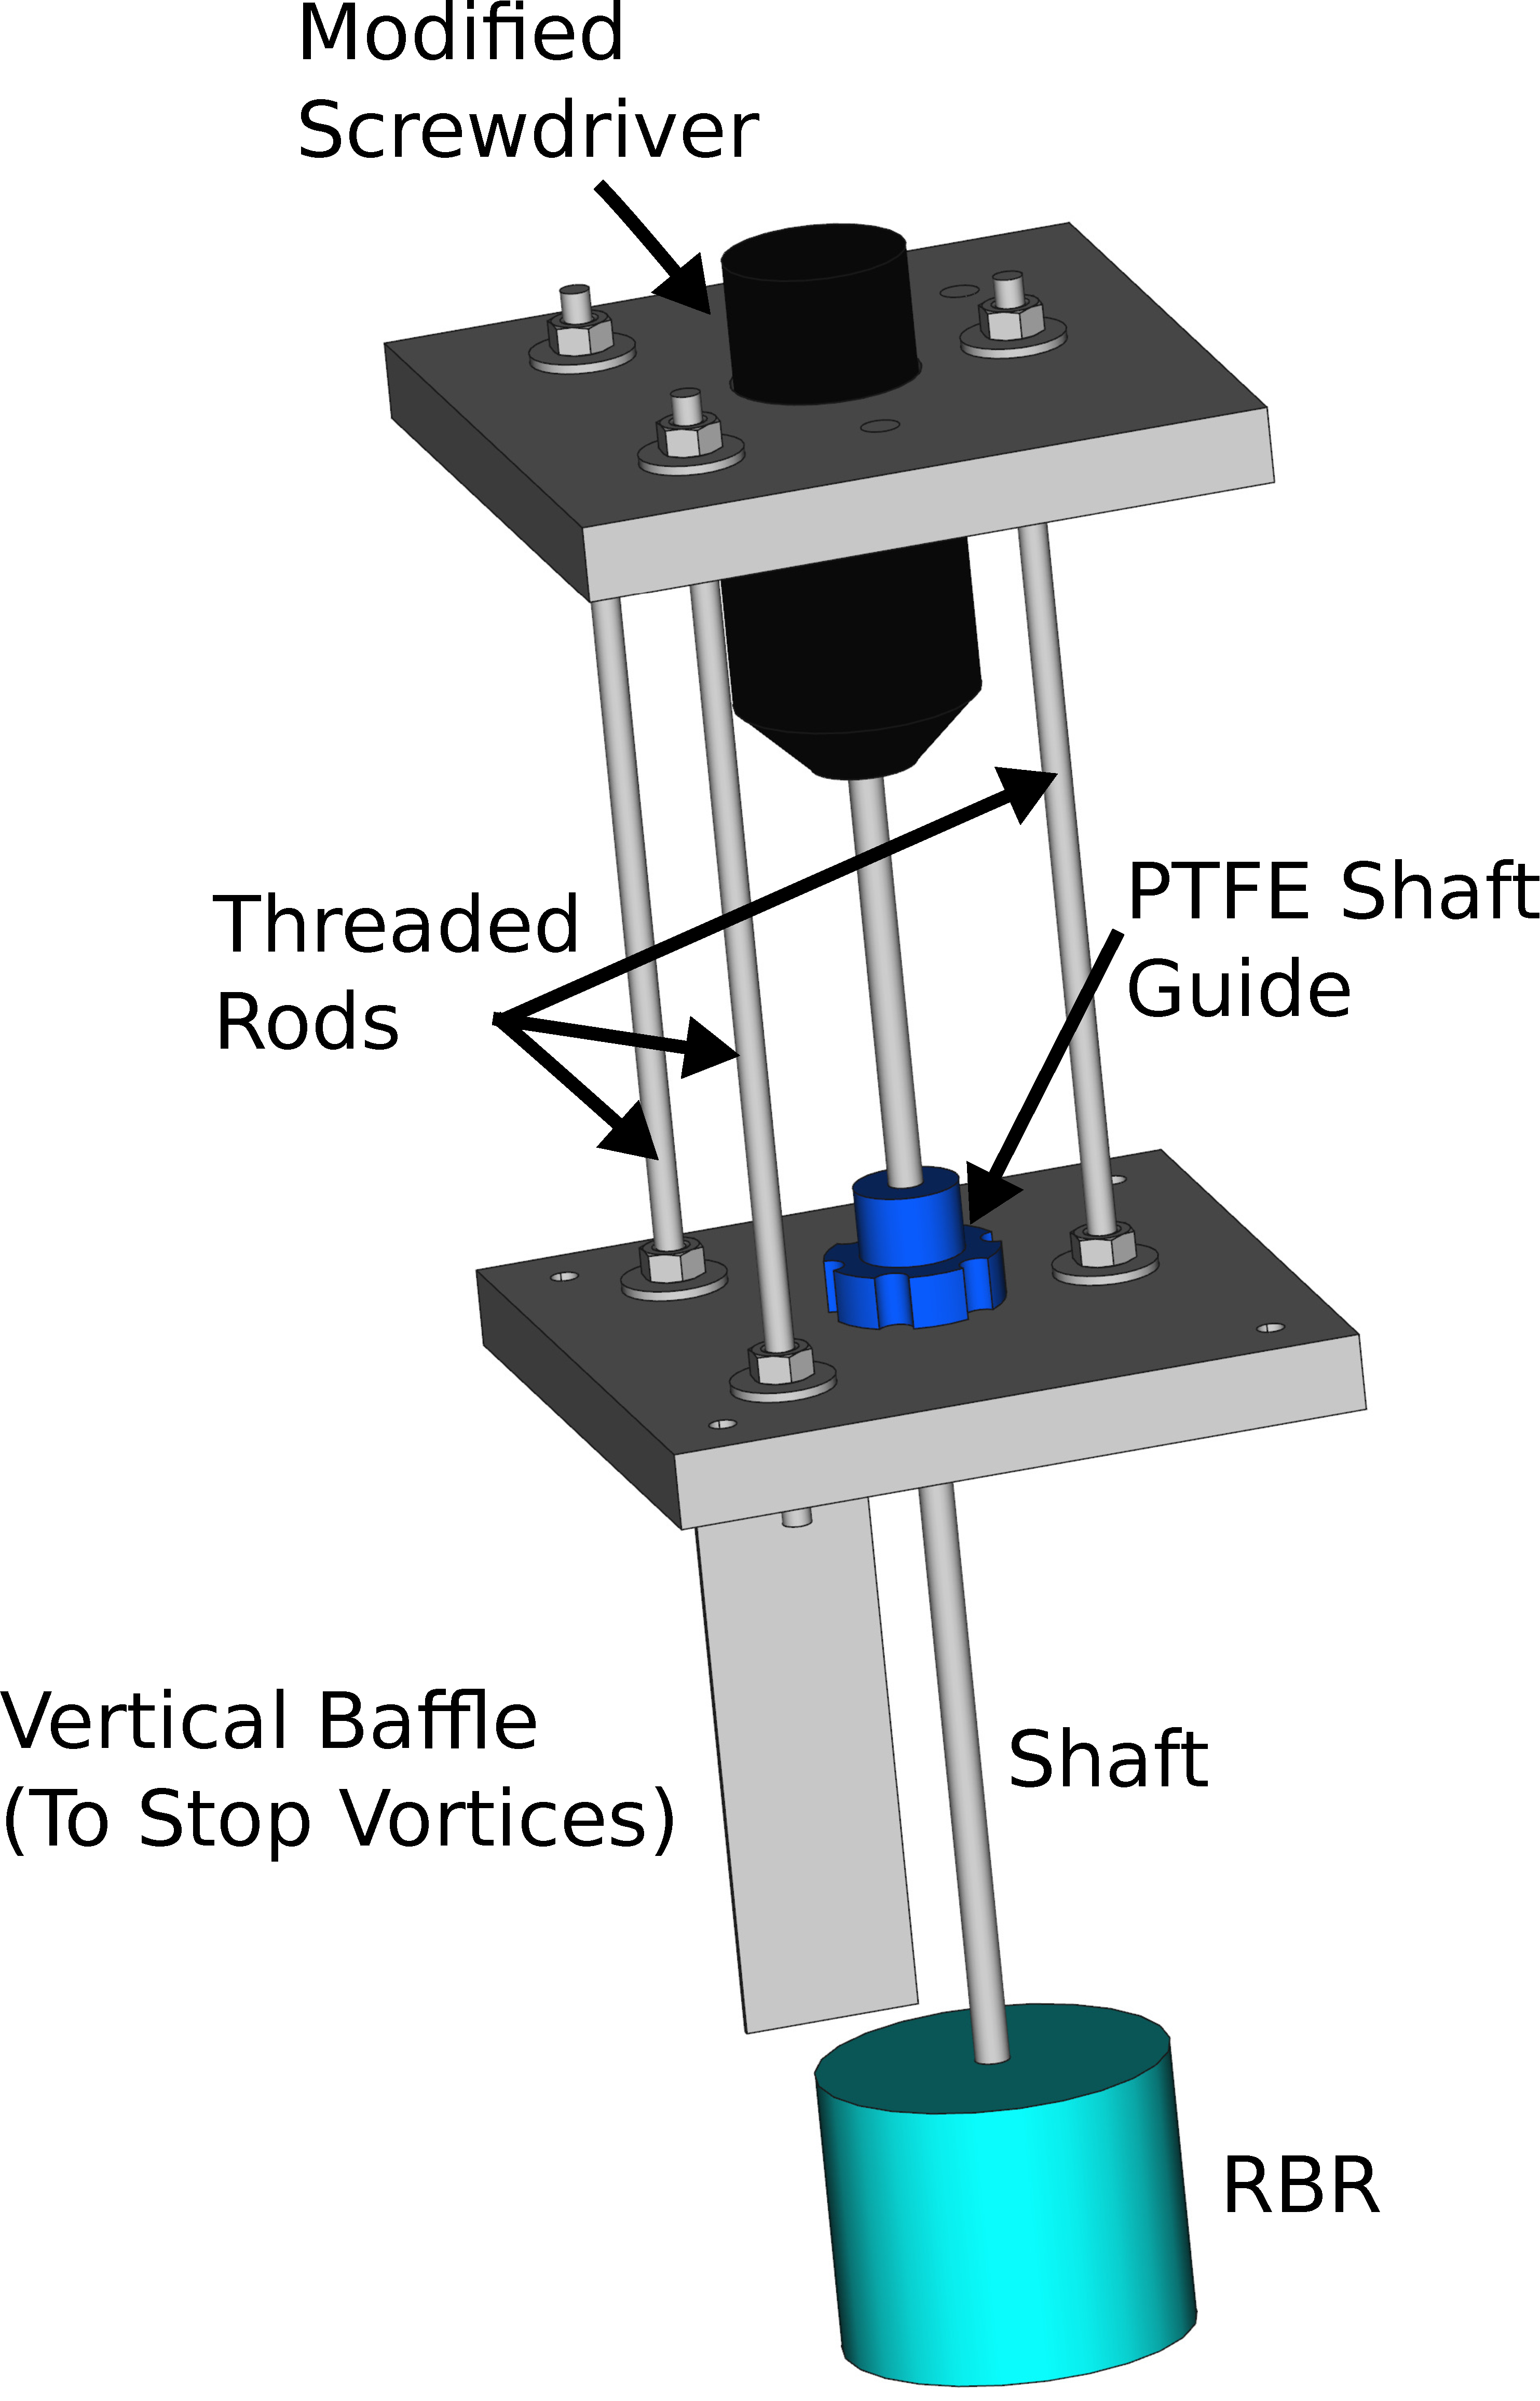
\includegraphics[width=0.5\textwidth]{RBR-moduleWithNotes}
  \caption{A RBR module with a drive assembly mounted at the top baffle,
    which in turn is mounted with adjustable threaded rods to the lower baffle. This houses the shaft guide for the RBR axle. The lower baffle mounts to the
    top of the platform, and on the RBR modules underside sits a wave baffle.}\label{fig:rbr-module}
\end{figure}

The upper baffle can be height adjusted, in order to easily calibrate the desired depth of the RBR. It is ideal to have the RBR distanced from the water surface. It is preferred to have it at a lower level than the bottom of the pontoons to prevent air reaching the RBR. 

The speed of the RBRs can be controlled remotely. The rotational speed interval of the RBR ranges from 0 to 600 rpm, where 500~rpm is ideal.


The RBR modules can be attached to the intended slots on the platform. The modules should be oriented such that the vertical baffle is parallel to the travel direction to minimize the vehicles water friction. Fly nuts are used to hold the modules in the slots. 

\subsection{Propulsion}
The propulsion is made from air-propellers, installed in an acrylic plastic protection housing. Acrylic plastic rudders were installed in front of the propellers, these are controlled through a single servo located at the back of the platform. The layout of the propulsion mechanism is shown in \cref{fig:propellerWithNotes}.

\begin{figure}[h]
   \centering
   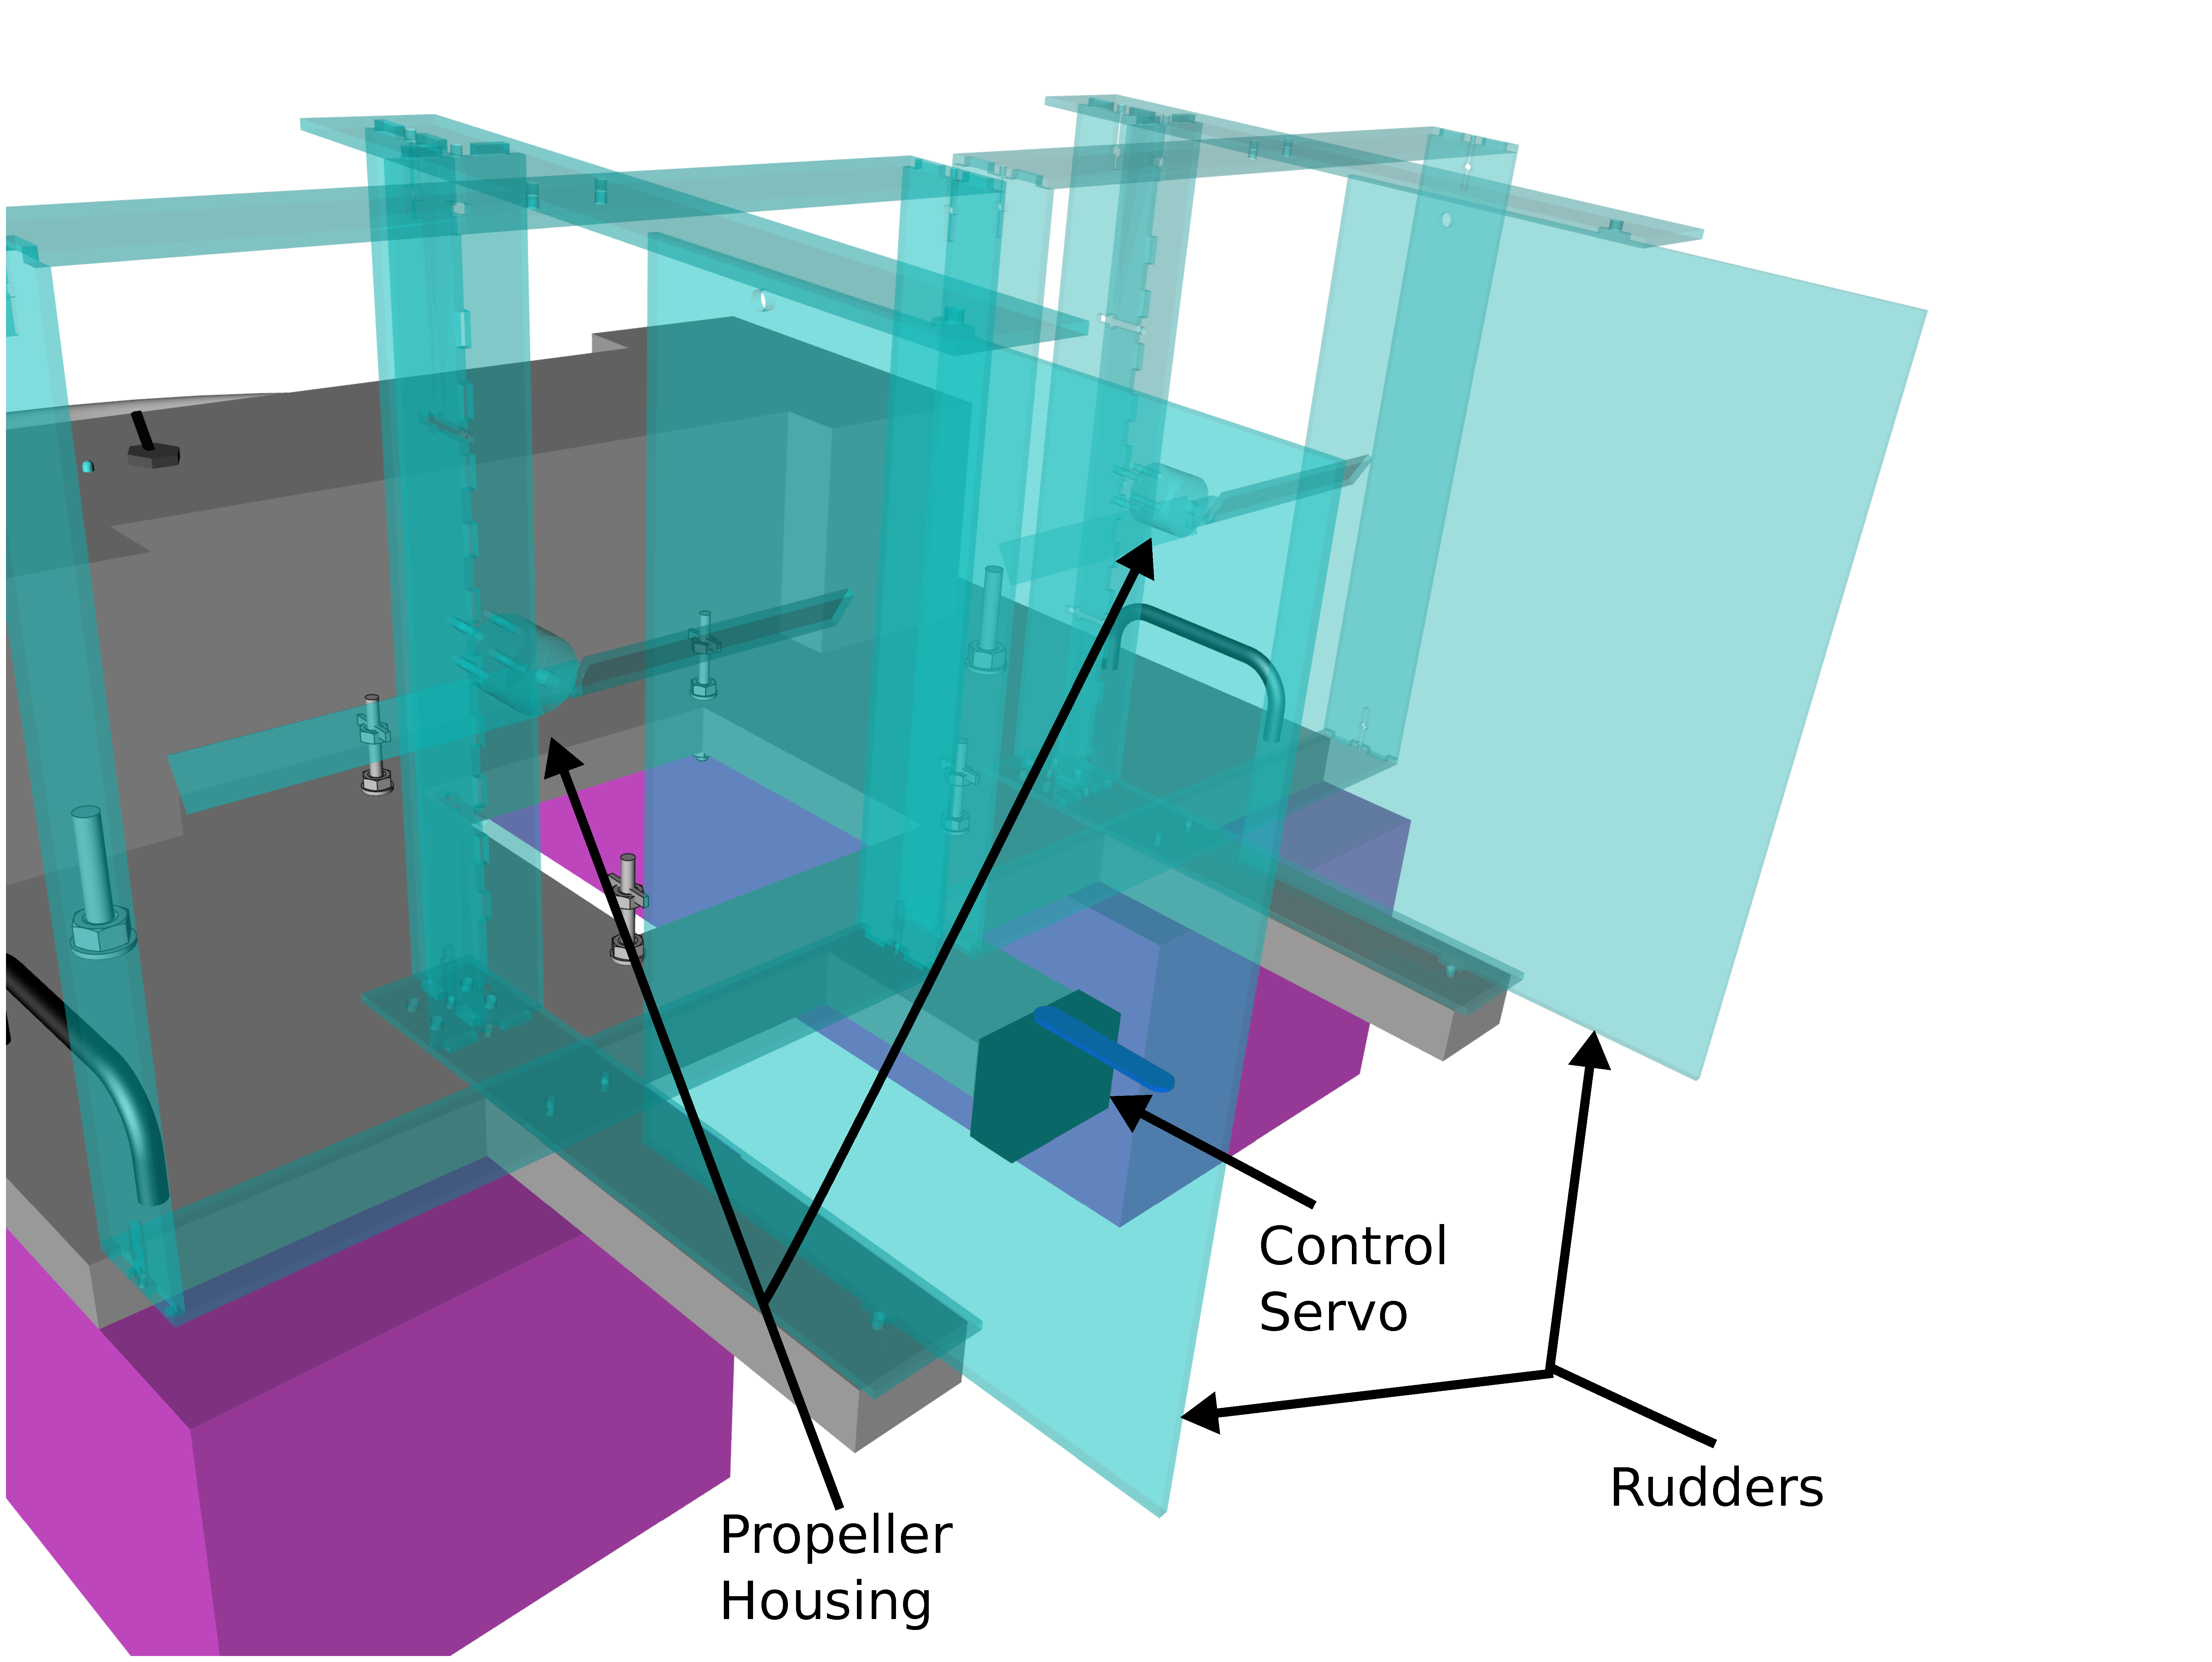
\includegraphics[width=.75\textwidth]{propellerWithNotes}
   \caption{The propulsion construction.}
   \label{fig:propellerWithNotes}
\end{figure}

\subsection{Water protection}

An acrylic protection cover were manufactured in order to protect the batteries, the engine control units, and other electronic equipment. Two separate acrylic covers were also constructed to protect the drive assemblies of the RBR modules. The covers do not protect the equipment from submersion, only from small splashes or rain. To install the covers, just place them over the RBR modules. The cover for the electronics is held in place with one screw on either side of the electronic enclosure.

\subsection{Transportation}

To ease transportation, the weight of the platform can be reduced. This is done by first removing the protective covers, followed by disconnecting the power cables connected to the batteries and RBR drive assembly. It is then possible to remove the batteries and RBR modules from the platform. During transport care needs to be taken such that the propulsion mounts are not damaged, as these parts are fragile.
\clearpage
\section{Radio Controller}
The radio controller used to control the vehicle is a Radiolink AT9 9 channel
2.4GHz control system. The controller supports the provided Radiolink R9D
9 channel, 2.4 GHz DSSS (Direct-sequence spread spectrum) receiver.

\subsection{Steering}
The Layout of the buttons on the controller can be seen in
\cref{fig:controller_front} and \cref{fig:controller_back}, for the front and
back of the controller respectively. In \cref{fig:controller_front} the
\textit{Elevator/Rudder stick} is used to control the speed of propellers
driving the vehicle forward. The propellers will not move when the stick is in the
lowest position in the figure, and will have max speed when the stick is in the
top most position in the figure. Note that the stick should be put in the
lowest position when the electronics of the vehicle is powered on. Be careful to not run the propulsion motors too hard, as they tend to overheat.

The \textit{Throttle/Aileron Stick} is used to control the air rudders. Moving
the stick to the right will turn the vehicle to the right and moving it to the
left will turn it left.

The stick on the back of the controller, the \textit{VRC SW} stick in
\cref{fig:controller_back} is used to control the rotational speed of the RBRs.
If the stick is in the bottom most position the RBRs will not rotate. By moving
the stick upwards the speed will increase until the stick is in the top
position. Be sure to move the stick slowly when accelerating the RBRs, otherwise the top speed might not be reached.

\begin{figure}[h]
   \centering
   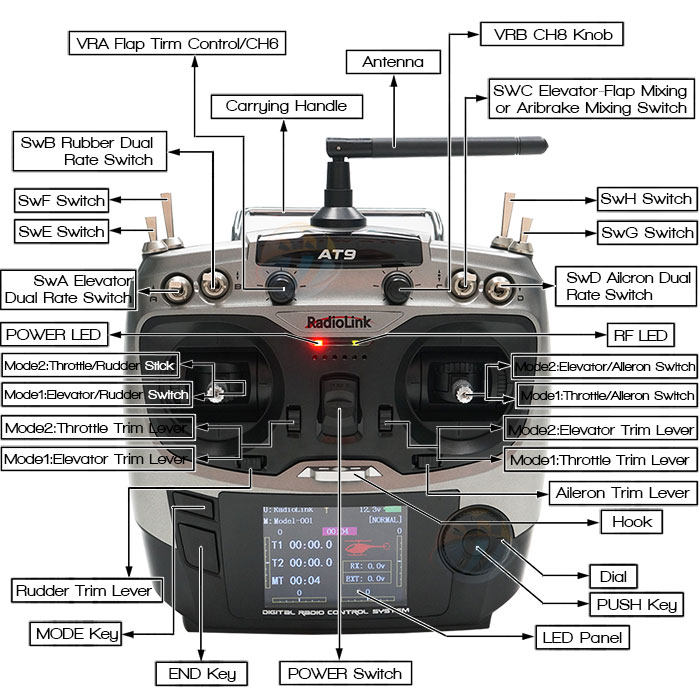
\includegraphics[width=.75\textwidth]{controller_front}
   \caption{The front of the radio controller, together with its buttons.}
   \label{fig:controller_front}
\end{figure}

\begin{figure}[h]
   \centering
   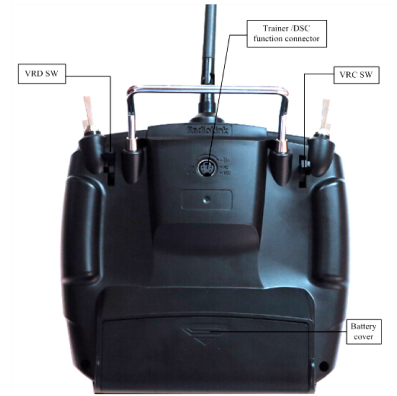
\includegraphics[width=.75\textwidth]{controller_back}
   \caption{The back of the radio controller, together with its buttons.}
   \label{fig:controller_back}
\end{figure}

\subsection{Settings}
When it comes to the controller settings, the base settings of the Helicopter type was used, which can be found under \textit{Model sel.} in the basic
menu of the controller. The basic menu is found by holding in the \textit{mode}
button.

Some settings however were changed to be able to maneuver the vehicle
more easily. The first of these setting tweaks were to put channel 1-3 from
normal to reversed, in order to get the buttons to behave in a way better
suited for a vehicle. This is done in \textit{reverse}, which can be found in the
Basic menu. In order to get the \textit{VrC SW} button on the back of the
controller, used to control the rotational speed of the RBRs (see
\cref{fig:controller_back} for button layout), one has to go into
\textit{AUX-CH} in the basic menu and choose which channel on the receiver one want to couple
it with. Then select \textit{VrC} on that channel. We chose to use channel 5,
but any other channel can be used as well.

\clearpage
\section{Electronics}

\begin{figure}[h]
   \centering
   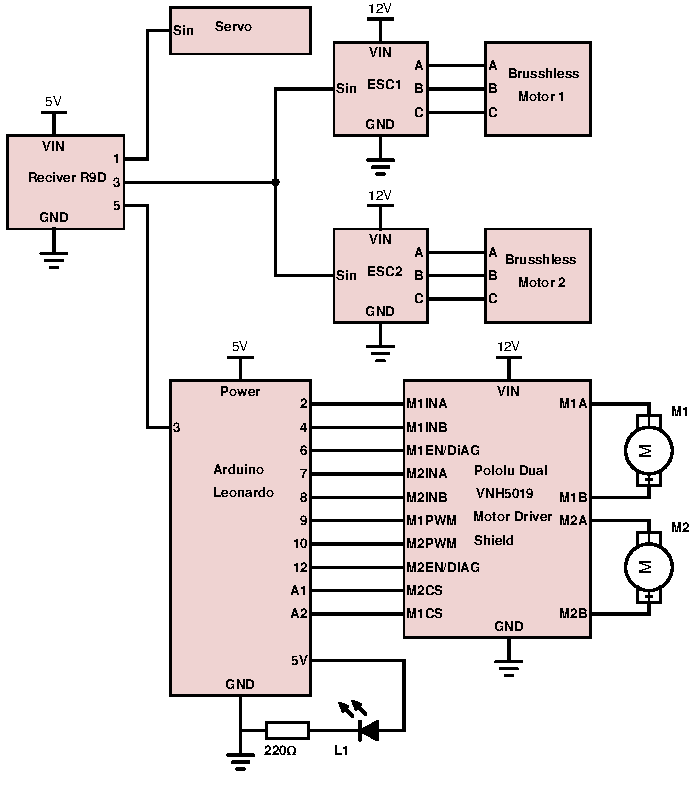
\includegraphics[width=.75\textwidth]{circuit}
   \caption{The circuit diagram of the electronics installed in floating platform.}
   \label{fig:circuit}
\end{figure}

\clearpage
\subsection{Thoughts Behind Construction and Suggested Improvements}
%\subsection{Floating Platform}
The reason why XPS was chosen is that it is cheap, offers good buoyancy, is easy to form, enduring, does not absorb water, and is easy to access in hardware and construction stores. However, it is not the most beautiful material, and could thus be exchanged for a lighter weight material like hollow aluminium. A sealed aluminium construction would be buoyant.

As for the main platform, it was constructed from glulam. The main advantages with glulam is that it is durable, cheap, recyclable, does not sink, and it offers a steady platform which is easy to work with. A disadvantage is that glulam is heavy.


%The initial design for the vehicle was a simple platform with two pontoons, one on either side, and that all other components would be mounted on top of this platform.  The pontoons are constructed from XPS cell foam, which is available in hardware and construction stores. The advantage of XPS over e.g. EPS foam, while more expensive, is that the material is denser and doesn’t absorb water. Cell foam is easy to form and work with, non-hazardous, and offers excellent buoyancy.

%As the development progressed, the load that the platform would be required to bear was roughly estimated and served as a basis for the size of the pontoons. They were estimated to displace 20 kg with some margin to the water surface. The platform itself, constructed from glulam wood, was attached to the pontoons with 10 mm threaded rods. An advantage with wood is that it doesn’t sink, is recyclable, cheap, and easy to work with using simple tools. A disadvantage with wood is that it’s heavy. A hollow aluminium construction, e.g. sealed square tubing, could also be buoyant, and offer lighter weight.

To distribute weight as evenly as possible, the RBR modules were placed at either end in the open space between the pontoons, and the batteries were placed above the center of each pontoon. The batteries were placed in a slot in the platform, above the center of each pontoon, to reduce weight, lower center of gravity and increase stability. The available space for electronics was thus limited to the middle of the platform, between the RBR modules.

To improve deflection of head on collisions, a rounded front bumper was added which also serves as a means of adding distance between the platform and any side obstacles. Without this bumper, the vehicle could be hard to manoeuvre in tight spots.

\subsubsection{RBR modules}

The main thought for the RBR modules were to have them as a separate product on the vehicle. This will not just make transportations easier, it will also simplify replacements of the reactants in the RBR. By having a set of four RBR modules it is easy to just replace the modules with used up reactants with new modules. This allows the vehicle to continue cleaning the water while the reactant is changed in the removed modules.

The reason why a screwdriver was modified and chosen as motor for the RBR is that it is cheap, provides a suitably strong DC-motor, and comes with a rugged chuck which is insensitive to off-axial loads (non-axial forces like roll forces, and forces from a not perfectly lined up construction). The chuck also makes it easier to remove the RBR axle from the drive assembly. A disadvantage of using a modified screwdriver is that a custom mount had to be manufactured. Another disadvantage was that an Arduino with motor controller shield, which in turn needed a separate 5~V line, was needed to power and control the screwdriver motors via RC. This is a somewhat complicated solution, but relatively cost effective.



%On the top baffle of the RBR module we have attached a modified screwdriver to drive and attach a RBR with a shaft. The choice to use a screwdriver was to reduce cost, as it provides a suitably strong DC-motor together with a rugged chuck which is insensitive to off-axial loads (non-axial forces like roll forces, and forces from a not perfectly lined up construction). It also speeds up disassembly of the RBR axle from the drive assembly. A disadvantage of using a modified screwdriver is that a custom mount had to be manufactured. Another disadvantage was that an Arduino with motor controller shield, which in turn needed a separate 5~V line, was needed to power and control the screwdriver motors via RC. This is a somewhat complicated solution, but relatively cost effective.


%To modularize the construction, we choosed that the RBRs should be self-contained with drive assembly and wave baffles in a module. This has the advantage of reducing the weight of the platform for transport and reducing the transport dimensions. Furthermore, the modularization gives the advantage that multipe RBR modules can be built and speed up the refill process when changing the reactant inside the RBR. If one has four RBR modules the unused modules can be preloaded and one only has to change the modules when refilling, maximizing the time the vehicle can spend cleaning the environment. It also allowed development and initial testing of the drive assembly and measurements of power consumption without a finished floating platform.

%Both baffles, with shaft guide and drive assembly is mounted above the surface, with only the RBR axle and RBR protruding below the surface. To reduce the formations of vortices induced by the rotation of the RBR, a wave baffle was mounted along the RBR axle to stop air from reaching the RBR.

\subsubsection{Propulsion}

At an early stage of development, it was chosen in consultation with an RC-expert that we should use air-propellers for propulsion, as they perform better than water propellers at lower speeds. The advantages of this is simplicity of construction, cost effectiveness, and that water-electricity contact concerns are more easily managed. Furthermore air propellers will not stir up the bottom of a lake, and thus not affect the water cleaning properties of the vehicle.

Disadvantages of water propellers, such as motors intended for electric RC-boats, are that they have poor low speed manoeuvrability. Disadvantages of air-propulsion are the bulkier form factor, as bigger rudders and propellers are needed to propel the vehicle. There is also a safety concern as air propellers are more likely to get in contact with hands, hair, and other vulnerable body parts. To prevent some of these possible incidents to happen, an acrylic plastic frame were installed around the propellers. A further improvement would be to enclose the propellers in a rigid mesh.

%We chose to use two air propellers mounted in the rear of the platform together with two large rudders controlled by a single servo, the control of which is described in the controller section. The complete motor-rudder assembly was laser cut from acrylic glass which is a cheap, low weight material. However, the assembly proved to be a bit fragile, and some care was needed when handling the floating platform, to prevent damaging any of the delicate parts. Schematics and design plans can be found in \cref{sec:appendix-a}.

\subsubsection{Water Protection}
While the covers over the RBR modules and electronics helps deflect smaller water splashes from reaching the electronics, it is probably not enough to fully protect the vehicle from heavy rain, or being submerged into the water. Should the equipment be in need of better protection, the electronic equipment could be mounted in an IP classified enclosure. This was not done because of budget restrictions.

\clearpage
\section{Large scale test using a pH-indicator and sodium hydroxide}

\subsection{Background}
From the beginning it had been suggested by SpinChem\textsuperscript{\textregistered} that a large scale test with the finished product should take place. The test was supposed to be performed using water resembling that of a mining pond with all of its usual pollutants. The vehicle should, in this volume, be manoeuvred while carrying one or more RBRs loaded with a suitable material. A suitable material would be one that is capable of adsorbing the pollutents of interest.

After reconsideration, SpinChem\textsuperscript{\textregistered} decided it would be a bad idea to create a larger volume of heavy metal polluted water. In the case that it could not be fully recovered, it would be both tedious and expensive to dispose of the polluted water. The volume for the large scale experiment was set to be 2 m$^3$.

\subsection{Method}
Instead of using polluted water it was suggested to perform a simpler, more environmental, visual test using either a coloring agent called allura red, and purify it by loading the RBR with active carbon (AC). This process would color the water red, and when the colored water is forced through the rotating RBR, the allura red would slowly be adsorbed by the AC, making it less red as more and more water gets treated. This process would take a considerable amount of time, but in return it has the benefit of restoring the water to practically the inital conditions as it were before adding the allura red.
 
The other alternative would be to use the pH-indicator phenolphthalein in combination with a base (NaOH) which would dye the water pink when the pH gets above 8. For the test with the phenolphthalein the reactor chambers would be loaded with cation-exchange resins amberlite (CER). The phenolphthalein would be added to the 2 m$^3$ of water. This by itself would however not induce a change of color in the water. Only when adding enough NaOH to force the pH above 9, the phenolphthalein would give off a pink color. The CER in the RBR would neutralize the base until the pH drops below 9, and thereby shifting the color of the water back to colorless. This process would not require the full volume of water to be treated by the RBR, it would only require that enough particles, in the total voulume, is adsorbed by the CER in order to lower the pH below 8 in the total volume. The concerns when using the CER approach would be the amounts of phenolphthalein required for reflecting a strong enough coloring in the final volume, since the phenolphthalein itself will not be adsorbed.

Compared to the AC process this method is very fast. However the water will not be completly restored after just neutralizing the NaOH. Since the phenolphthalein does not get adsorbed itself, it is necessary to inspect whether or not phenolphthalein would be okay to dispose of in regular sewers. It turned out that phenolphthalein poses no danger as a marine pollutant\cite{url}, all the same it would be best to use as little as possible.
After careful considerations, it was decided to perform the large scale test using the CER approach.

\subsection{Experimental set up}
A fixed volume of 150~ml distilled water, mixed with a fixed amount of 150~$\mu$l 1~M NaOH was prepared before each run. The start concentration of phenolphthalein in the prepared mixture was set to $0.05$~mg/l. For each new testrun the concentration was halved until the pink color no longer appeared before the naked eye. The final concentration of phenolphthalein needed was a mere $0.78$~percent of the start concentration. To scale up to the final volume of 2~m$^3$ it would only require $0.78$~g of pure phenolphthalein. The final concentration would be $1.225$~$\mu$M (see \cref{sec:calculations}).

With a known minimum amount of phenolphthalein required, the process of minimizing the amount of needed NaOH could begin. With a fixed amount of phenolphthalein ($0.78$~percent of start concentration) in the same amount (150~ml) of distilled water, 1~Molar NaOH was added a few $\mu$l at a time until a pink color was visible. Scaling up to the final volume of 2~m$^3$ revealed that it would require $3.5$~L of 1~M NaOH for the final test.

\subsection{Distilled vs. tapwater}
Since all of the minor tests had been performed using distilled water instead of tap water, which would be used in the large scale test, there was a need to redo the previous experiments with tap water. When testing the amounts of NaOH needed, it seemed as though it required more NaOH the first run compared to the rest of the runs. Since we did not want to waste phenolphthalein, the same water was used for the following test, the only differences were that a RBR loaded with CER had been used to neutralize the NaOH in between.

The theory behind it is that the initial pH is lower than the pH where the pH-indicator turns from pink to colorless. Meaning that for the first test the initial pH is around 6-7 while the later tests starts at an initial pH of 8-9, thus requiring smaller amounts of NaOH.
Comparing the initial pH between distilled water and tapwater showed that distilled water had somewhat lower pH. After running the CER loaded RBRs without any added base, there was a slight decrease in pH in both the distilled water and tapwater. The decrease was however larger in tapwater when comparing to the start pH value.
The new test showed that it would require a small increase of phenolphthalein from $0.78$~g up to $1.17$~g. The NaOH was increased by a tenfold.

\subsection{Scaling up}
When testing in larger scales of 5~L and 70~L it became clear that the amount of base needed, in order to visually detect a pink color, decreased exponentially. When testing with 70~L it only required 20~ml instead of the expected 120~ml, which was calculated from the 150~ml experiments.

In the final volume of 2~m$^3$ it only required 150~ml of 1~M NaOH to turn the entire volume pink. This can be explained by Lamberts law which explains that there is an exponential correlation between the transmission of light through a substance, the product of the absorption and the length the light passes through the material.\cite{pierre}

\subsection{Calculations}\label{sec:calculations}
The first calculations for phenolphthalein using distilled water:
$1.17$~ml of $0.05$~mg/ml phenolphthalein was needed in a total volume of $0.150$~L:
\begin{equation}\label{eq:concentration}
    1.17 \text{ ml} \times 0.05 \text{ mg/ml}
    = 0.0585 \text{ mg} = 0.0000585 \text{ g} \text{ phenolphthalein per } 0.150 \text{ ml}.
\end{equation}

The final volume is $2000$~dm$^3$, upscaling from $0.150$~dm$^3$:
\begin{align}
x \times 0.150 \text{ dm}^3 &= 2000 \text{ dm}^3 \nonumber \\
x &= \frac{2000 \text{ dm}^3}{0.150 \text{ dm}^3} \approx 13333.33 \\
0.00117 \text{ L} \times 13333.33 &\approx 15.6 \text{ L phenolphthalein.} 
\end{align}
For the final volume of 2000~dm$^3$, there should be $15.6$~L of the $0.05$~mg/ml phenolphthalein solution.
To simplify it is practical to recalculate this into how many grams of the substance we need instead:
\begin{equation}
    15.6 \text{ L} \times 0.05 \text{ mg/ml} = 0.78 \text{ g}.
\end{equation}

To put this in concentrations for the final volume of 2000~dm$^3$:

\begin{align}
    \text{volume } V &= 2000 \text{ dm}^3 \\
    \text{molarmass phenolftalein } M_p &= 318.3228 \text{ g/mol} \\
    \text{mass } m &= 0.78 \text{ g} \\
    \text{moles } M &= \frac{0.78 \text{ g}}{318.3228 \text{ g/mol}} \approx 0.00245 \text{ mol} \\
    \text{concentration } c &= n/V = 0.000001225 \text{ mol/dm}^3 = 1.225 \mu\text{M}
\end{align}

The final amount of phenolphthalein used was calculated in the same manner as before where the only difference were that instead of $1.17$~ml of the $0.05$~mg/ml phenolphthalein solution there was $1.755$~ml.
This implies that the final concentrations increased as well but it is still in the vicinity of a few $\mu$M.

For the NaOH the calculations are not really important since most of the time it was just to pour until the water-mass started taking a pinkish color. The amounts changed drastically with every upscale performed. In the end it required 150~$\mu$l 1~M NaOH to color 2000~dm$^3$.

\subsection{Results and discussion}
After performing a few test runs, and adjusting the amount of NaOH, we managed to reduce the time needed to decolor the 2~m$^3$ water from 25 to 10~minutes. The floating platform carrying two rotating RBRs loaded with CER was manoeuvred remotely around the pool. During the test it was clearly visible how the water just beneath the platform, around the RBRs, lost its pink color.
We had guessed in advance that it would take up to 45-60 minutes to decolor the volume. The fact that it only took 10~minutes was beyond expectations.

\subsection{Conclusion}
The SpinChem\textsuperscript{\textregistered}'s patterned RBR can be put on floating constructions and be remotely manoeuvred in order to purify larger volumes of polluted water. This can be done within reasonable time frames. These tests supports the possibility to load the reactors with other materials in order to specifically adsorb certain kinds of pollutants. It has the potential to purify water without having a negative effect on the environment.

\clearpage
%\section{Compliance to specification}

The specification of requirements \ref{kravspec} outlined several objectives of this project. How well the requirements are fulfilled can be seen in Table \ref{tab:kravspec} below.

\todo{Kolla om dimensonerna på flotten stämmer}

\FloatBarrier
\begin{table}[H]
\center
\caption{The requirements shown in \ref{kravspec}, together with how well they are fulfilled}
\begin{tabular}{l p{0.28\linewidth} l}
\toprule
\rowcolor{lightgray}
Requirement & Complience\\
\midrule
1 (a) &  Not tested but assumed to function properly\\
\midrule
1 (b) &  The RBRs needed to be adjustable, and are also constucted that fashion \\
\midrule
1 (c) &  The constructed vehicle is 60x90 cm, this makes it larger than in the specifications \\
\midrule
2 (a) &  The vehicle only use electricity as fuel \\
\midrule
2 (b) &  Can be manoeuvred with a radio controller  \\
\midrule
2 (c) &  No occuring problems when the RBRs are rotating \\
\midrule
2 (d) &  Batteries are used, which can easily be removed and charged  \\
\midrule
2 (e) &  It should be easy to implement a autonomous operating system \\
\midrule
2 (f) &  Not tested but assumed to not be fulfilled \\
\midrule
3 &  Most of the parts are easily replicable, and there should not be a too hard to construct a new vehicle \\
\midrule
4 &  It is easy to remove the RBRs from the vehicle, as the RBR-modules are easy to remove from the platform. Should not be a problem to change the cleaning material \\
\midrule
5 (a)-(e) &  All listed materials have been tested and analysed \\
\midrule
6 &  A successful test was performed, with the local newspaper filming \\
\midrule
7 &  This objective was only partially completed, through video footage from different angles at the final tests. \\
\bottomrule
\end{tabular}
\label{tab:kravspec}
\end{table}


\begin{itemize}
	\item The ability to determine when the reactant has been consumed. This has been experimentally verified, but no measurement method has been developed.
	\item The outer dimensions of the vehicle exceeded those from the specification, but because of the modularization of the vehicle, with removable RBR modules and pontoons, the size remains manageable.
	\item There is no way to measure the remaining lifetime of the batteries, but this has been experimentally tested and is known to last long enough such that the reactants are consumed faster than the batteries are depleted.
	\item One optional objective was to get the vehicle to drive autonomously. Due to time restrictions this was never started as it was considered too time consuming. 
\end{itemize}
\clearpage

\appendix
\section{Materials and blueprints}

\subsection{Floating platform}

The floating platform is built up from the following parts:

\begin{itemize}
  \item 1 main plate made from 22~mm thick glulam wood. Observe that in the
    blueprint for this plate holes for cables, and screw holes for the
    propeller holder and circuit boards are not included. The front bumper,
    servo and containing straps for the batteries are screwed to this plate.
  \item 4 floating elements made from 70~mm XPS cell foam
  \item 2 boards that goes below the floating elements
  \item 4 250~mm M10 stainless steel threaded rods
  \item 8 70~mm M6 stainless steel threaded rods
  \item 4 M10 nuts
  \item 4 M10 lock nuts
  \item 16 M6 nuts
  \item 8 M6 wing nuts
  \item 8 M10 washers
  \item A 20~mm plastic tube bent to a quarter circle with a radius of 403~mm,
    with 100~mm extra material to attach in each end.
  \item 2 straps to keep the batteries in place
  \item 4 carry handles
  \item Self drilling screws, and washers used to attach electronics, battery
    straps, and bumper.
\end{itemize}

\subsection{Electronics}

\crefformat{footnote}{#2\footnotemark[#1]#3}

The electronic components mounted on the platform are:

\begin{itemize}
  \item 1 Arduino Leonardo
  \item 1 Dual VNH5019 Motor Driver Shield
  \item 2 2725 Brushless Outrunner Motors 1600kv
  \item 2 ESC who matches the brushless motors
  \item 2 plastic propellers
  \item 1 15~kg servo
  \item 1 R9D Radio Control Receiver
  \item 1 blue power-LED (mounted on the cover)
  \item 1 220~$\Omega$ resistor
  \item 1 power switch (mounted on the cover)
  \item 1 0.1 $\mu$F capacitor rated for at least 12V \footnote{\label{fotnot_app} These items can be replaced with a pre built 12~V to 5~V power supply. The electronics are connected according to the circuit diagrams, and the files in \texttt{RBR\_driver.zip} is loaded onto the Arduino.} \todo{Hårdkodade fotnoter (sorry!) så om vi har fler någonstans måste vi ändra}
  \item 1 22 $\mu$F capacitor rated for at least 5V \footnotemark[1]
  \item 1 L4940V5 linear regulator \footnotemark[1]
  \item Protoboard to build the 5~V PSU on \footnotemark[1]
  \item A few meter mains cable 2x1.50~mm$^2$ unshielded
  \item A few meter signal cable
  \item A few sensor cables and connectors (for servo, ESC, and power to RC
    receiver)
  \item Heatshrink tubing to cover connections
  \item A few blade receptacle 4.8x0.5~mm fully insulated, blade terminal red
    4.8x0.8~mm, ring cable lug 4.3~mm used to connect the cables together.
  \item A few 2.54~mm pin headers for the connections to the Arduino.
\end{itemize}

Note that the items marked with (*) can be replaced with a pre built 12~V to
5~V power supply.  The electronics are connected according to the circuit
diagrams, and the files in RBR\_driver.zip is loaded onto the Arduino.

\subsection{RBR modules}

Each of the two RBR modules are built up from:

\begin{itemize}
  \item 1 top plate made from a 22~mm thick board (observe that the holes for
    the 3D printed motor holder are not included.)
  \item 1 bottom plate made from a 22~mm thick board
  \item 1 3D printed motor holder
  \item 1 motor, shuck, and gearbox taken from a $\dots$
    screwdriver.\todo{Insert model here}
  \item 3 330~mm M10 stainless steel threaded rods
  \item 3 M10 locking nuts
  \item 9 M10 nuts
  \item 12 M10 washers
  \item 2 50~mm M4 stainless steel threaded rods
  \item 2 110~mm M4 stainless steel threaded rods
  \item 10 M4 washers
  \item 10 M4 nuts
  \item 4 long M3 screws
  \item 4 M3 nuts
  \item 4 M3 washers
  \item 1 shaft guide NS29
  \item 1 piece of 50~mm wide and 200~mm long piece of 2~mm stainless steel
    bent to form a baffle.
  \item 1 piece of metal to put pressure on top of the motor.
\end{itemize}


\subsection{Covers for RBR modules and electronics}

The cover for the RBR module are made from 5 pieces of 3~mm thick acrylic glass
glued together, with a handle attached on top. See blueprint.\todo{ref to blueprint}

The cover for the electronics are made from 13 pieces of 3~mm thick acrylic glass
glued together. On top of this cover the power switch is connected. This cover
was fastened to the platform using handmade angle brackets and a nut.



\end{document}

